%  $Description: Thesis
%  $Author: xxx $
%  $Date: xxx  $
%  $Revision: 0.0 $

\documentclass[11pt]{book}
\usepackage{iiit_thesis}
% \usepackage{times}
\usepackage{epsfig}
% \usepackage{amsmath}
% \usepackage{amssymb}
% \usepackage{latexsym}
\usepackage{graphicx}
% \usepackage{multirow}
% \usepackage{algorithm2e}

\usepackage{times}
\usepackage{latexsym}
\usepackage{physics}
\usepackage{amsmath}
\usepackage{amssymb}
\usepackage{stmaryrd}
% \usepackage{tikz}
\usepackage{multirow}
\usepackage{multicol}
\usepackage{array}
\usepackage{amsthm}
\usepackage{mathtools}
\usepackage{booktabs}
% \usepackage{float} % use for H with figures, which forces figure locations. 

\newcommand\ddfrac[2]{\frac{\displaystyle #1}{\displaystyle #2}}
\newcommand{\N}{\ensuremath{\mathbb{N}}}
\newcommand{\coT}{\ensuremath{T^*}}
\newcommand{\Lie}{\ensuremath{\mathfrak{L}}}
\newcommand{\Vectorfield}{\ensuremath{\mathfrak{X}}}
\newcommand{\pushforward}[1]{\ensuremath{{#1}_{\star}}}
\newcommand{\pullback}[1]{\ensuremath{{#1}^{\star}}}
\newcommand{\vectorfield}{\ensuremath{\mathfrak{X}}}

\newcommand{\pushfwd}[1]{\pushforward{#1}}
\newcommand{\pf}[1]{\pushfwd{#1}}

\newcommand{\boldX}{\ensuremath{\mathbf{X}}}
\newcommand{\boldY}{\ensuremath{\mathbf{Y}}}
%\renewcommand{\UrlFont}{\ttfamily\small}
\newcommand{\card}[1]{\left| #1 \right|}
\DeclarePairedDelimiterX{\infdivx}[2]{(}{)}{%
 #1\;\delimsize|\delimsize|\;#2%
}


\newcommand{\infdiv}{D\infdivx}

\usepackage{amsmath}
\usepackage{amssymb}
\usepackage{amsthm}
% \usepackage{minted}
\usepackage{hyperref}
\usepackage{cancel}
% \usepackage{mathtools}

%\newcommand{\card}[1]{\ensuremath{\left| #1 \right|}}
\newcommand{\wtov}{\texttt{word2vec }}
\newcommand{\citep}[1]{\texttt{cite: #1}}
\newcommand{\citet}[1]{\texttt{cite: #1}}
\newcommand{\R}{\ensuremath{\mathbb R}}

\def\qed{$\Box$}
\newtheorem{theorem}{Theorem}
\newtheorem{corollary}[theorem]{Corollary}
\newtheorem{definition}[theorem]{Definition}
\newtheorem{lemma}[theorem]{Lemma}
\newtheorem{observation}[theorem]{Observation}
% \newtheorem{proof}[theorem]{Proof}
\newtheorem{remark}[theorem]{Remark}
\newtheorem{example}[theorem]{Example}


\graphicspath{{figures/}{./}} % To include images in other directories

\long\def\symbolfootnote[#1]#2{\begingroup%
\def\thefootnote{\fnsymbol{footnote}}\footnote[#1]{#2}\endgroup}
\renewcommand{\baselinestretch}{1.2}
\onecolumn
%--------------------------------------------------------

\begin{document}
\pagenumbering{roman}

%% TITLE PAGE
\thispagestyle{empty}
\begin{center}
\vspace*{1.5cm}
{\Large \bf Mathematical Structures for Word Embeddings}

\vspace*{3.75cm}
{\large Thesis submitted in partial fulfillment\\}
{\large  of the requirements for the degree of \\}

\vspace*{1cm}
{\it {\large Master of Science in Computer Science and Engineering by Research} \\
% {\large in\\}
% {\large COURSE \\}}
}

\vspace*{1cm}
{\large by}

\vspace*{5mm}
{\large Siddharth Bhat\\}
{\large 20161105 \\
{\small \tt siddharth.bhat@research.iiit.ac.in }}


\vspace*{4.0cm}
{\psfig{figure=figures/iiit.eps,width=14mm}\\}
% {\large CSTAR: Center for Security, Theory, and Algorithms Research \\}
{\large International Institute of Information Technology\\}
{\large (Deemed to be University) \\}
{\large Hyderabad - 500 032, INDIA\\}
{\large November 2021 \\}
\end{center}


%% COPYRIGHT PAGE
\newpage
\thispagestyle{empty}
\renewcommand{\thesisdedication}{{\large Copyright \copyright~~NAME, YEAR\\}{\large All Rights Reserved\\}}
\thesisdedicationpage

%% CERTIFICATE PAGE
\newpage
\thispagestyle{empty}
\vspace*{1.5cm}
\begin{center}
{\Large International Institute of Information Technology\\}
{\Large Hyderabad, India\\}
\vspace*{3cm}
{\Large \bf CERTIFICATE\\}
\vspace*{1cm}
\noindent
\end{center}
It is certified that the work contained in this thesis, titled `` '' by NAME, has been carried out under
my supervision and is not submitted elsewhere for a degree.

\vspace*{3cm}
\begin{tabular}{cc}
\underline{\makebox[1in]{}} & \hspace*{5cm} \underline{\makebox[2.5in]{}} \\
Date & \hspace*{5cm} Adviser: Prof. NAME
\end{tabular}
\oneandhalfspace

%%% DEDICATION PAGE
\newpage
\thispagestyle{empty}
\renewcommand{\thesisdedication}{\large To SOMEONE}
\thesisdedicationpage

\mastersthesis
\renewcommand{\baselinestretch}{1.5}

% ACKNOWLEDGEMENTS PAGE
\chapter*{Acknowledgments}
\label{ch:ack}

Acknowledgements goes here ...

%% ABSTRACT PAGE
\chapter*{Abstract}
\label{ch:abstract}

Abstract goes here ...



\tableofcontents
\listoffigures
\listoftables
%--------------------------------------------------------

\chapter{Introduction}
 
 

The popular opinion thanks to a confluence of distributional semantics
and machine learning is that systems such as \texttt{word2vec} learn
''vector representations''. This seemed to me to be confusing the encoding
the object (as a tuple of real numbers) with the algebraic structure
(that of a vector space). Hence, the modest goal of the thesis is an
attempt to disambiguate the term ``vector representations''.

Towards this end, we begin by surveying the algebraic structure of a vector
space, and what it would really mean if words were vectors. We then provide
a short explanation of the training mechanism of \texttt{word2vec}, and
discuss why the embeddings that are learnt by systems it and its ilk do not
deserve to be called vectors. 

Thereafter, we take a step back and start from scratch; what ought the axioms
be? Starting from a purely linguistic approach, we are led to conjecture, following
the seminal work of montague, that a set-based representation ought to be
the best representation possible.

Following an empirical approach, we attempt to generalize the success
of \wtov and the newly developed theory of contrastive losses, where we conjecture
that a Lie group representation ought to be the best representation possible.

We report on experiments performed on both of these representations, always
explained through the dual lenses of linguistics and abstract algebra. We hope
that this blend of perspectives provides fresh insight into representation
learning for NLP.

\chapter{Are words vectors?}

\section{\wtov}

The core training loop of \wtov (trained using negative sampling, in skip-gram
mode) involves attempting to learn \emph{two} representations for a given word,
called as the positive representation and the negative representation.

% \begin{minted}{py}
% def learn(lix: int, rix:int, larr:np.array, rarr:np,array,
%     out :float, target: float):
%     # gradient descent on loss (target - out)^2 where
%     # out = larr[lix] . rarr[rix ]
% def train(corpus):
%   poss = np.array((VOCABSIZE, DIMSIZE))
%   negs = np.array((VOCABSIZE, DIMSIZE))
% 
%   for wix in range(len(corpus)):
%     w = poss[corpus[wix]]
%     l = max(wix-WINDOWSIZE, 0)
%     r = min(wix+WINDOWSIZE, len(corpus)-1)
% 
%     for xix in range(l, r+1):
%         x = poss[xix]
%         out = np.dot(x, w)
%         learn(lix=wix, rix=xix, larr=poss, rarr=poss, out=out, target=1.0)
% 
%     for _ in range(NNEGSAMPLES)
%         xix = random.randint(0, len(corpus)-1)
%         x = negs[xix]
%         out = np.dot(x, w)
%         learn(lix=wix, rix=xix, larr=poss, rarr=negs, out=out, target=0.0)
%     
% \end{minted}


\section{Testing regime}

\section{Interpretations}



The output of the training regime are popularly interpreted as vectors. However,
we augment this discussion by bringing in nuance. In particular, we note that:
\begin{itemize}
\item Scalar multiples of the same vector represent the same concept as per the testing regime.
\item Vector addition has no clear meaning in the representation.
\item The identity element (the zero vector) holds no semantic meaning in the representation.
\item The reality of the training regime as-implemented makes it unclear as to
      what mathematical object is being learnt.
\end{itemize}

The classic explanation of `word2vec`, in skip-gram, with negative sampling,
in the paper and countless blog posts on the internet is as follows:

\section{Popular misconceptions}
% \begin{minted}{cpp}
% while(1) {
%    1. vf = vector of focus word
%    2. vc = vector of context word
%    3. train such that (vc . vf = 1)
%    4. for(0 <= i < negative samples):
%            vneg = vector of word *not* in context
%            train such that (vf . vneg = 0)
% }
% \end{minted}

% TODO: fix the wikipedia implementation
% Indeed, if I google "word2vec skipgram", the results I get are:
% - [The wikipedia page which describes the algorithm on a high level](https://en.wikipedia.org/wiki/Word2vec#Training_algorithm)
% - [The tensorflow page with the same explanation](https://www.tensorflow.org/tutorials/representation/word2vec)
% - [The towards data science blog which describes the same algorithm](https://towardsdatascience.com/word2vec-skip-gram-model-part-1-intuition-78614e4d6e0b)
% 
% The list goes on. However, __every single one of these implementations is wrong__.

The original \wtov \texttt{C} implementation does not do what's explained above,
and is drastically different. Most serious users of word embeddings, who use
embeddings generated from \texttt{word2vec} do one of the following things:

\begin{itemize}
\item They invoke the original C implementation directly.
\item They invoke the \texttt{gensim} implementation, which is
\emph{transliterated} from the C source to the extent that the variables names
are the same.
\end{itemize}

\section{The C implementation}

The \texttt{C} implementation in fact maintains \emph{two vectors for each word}, one where
it appears as a focus word, and one where it appears as a context word.
(Is this sounding familiar? Indeed, it appears that GloVe actually took this
idea from `word2vec`, which has never mentioned this fact!)

The setup is incredibly well done in the C code:

- An array called `syn0` holds the vector embedding of a word when it occurs
  as a \emph{focus word}. This is random initialized.

% \begin{minted}{cpp}
% https://github.com/tmikolov/word2vec/blob/20c129af10659f7c50e86e3be406df663beff438/word2vec.c#L369
%   for (a = 0; a < vocab_size; a++) for (b = 0; b < layer1_size; b++) {
%     next_random = next_random * (unsigned long long)25214903917 + 11;
%     syn0[a * layer1_size + b] =
%        (((next_random & 0xFFFF) / (real)65536) - 0.5) / layer1_size;
%   }
% \end{minted}

Another array called \texttt{syn1neg} holds the vector of a word when it occurs
as a \emph{context word}. This is zero initialized.

% \begin{minted}{cpp}
% https://github.com/tmikolov/word2vec/blob/20c129af10659f7c50e86e3be406df663beff438/word2vec.c#L365
% for (a = 0; a < vocab_size; a++) for (b = 0; b < layer1_size; b++)
%   syn1neg[a * layer1_size + b] = 0;
% \end{minted}

- During training (skip-gram, negative sampling, though other cases are
  also similar), we first pick a focus word. This is held constant throughout
  the positive and negative sample training. The gradients of the focus vector
  are accumulated in a buffer, and are applied to the focus word
  \emph{after} it has been affected by both positive and negative samples.

% \begin{minted}{cpp}
% if (negative > 0) for (d = 0; d < negative + 1; d++) {
%   // if we are performing negative sampling, in the 1st iteration,
%   // pick a word from the context and set the dot product target to 1
%   if (d == 0) {
%     target = word;
%     label = 1;
%   } else {
%     // for all other iterations, pick a word randomly and set the dot
%     //product target to 0
%     next_random = next_random * (unsigned long long)25214903917 + 11;
%     target = table[(next_random >> 16) % table_size];
%     if (target == 0) target = next_random % (vocab_size - 1) + 1;
%     if (target == word) continue;
%     label = 0;
%   }
%   l2 = target * layer1_size;
%   f = 0;
% 
%   // find dot product of original vector with negative sample vector
%   // store in f
%   for (c = 0; c < layer1_size; c++) f += syn0[c + l1] * syn1neg[c + l2];
% 
%   // set g = sigmoid(f) (roughly, the actual formula is slightly more complex)
%   if (f > MAX_EXP) g = (label - 1) * alpha;
%   else if (f < -MAX_EXP) g = (label - 0) * alpha;
%   else g = (label - expTable[(int)((f + MAX_EXP) * (EXP_TABLE_SIZE / MAX_EXP / 2))]) * alpha;
% 
%   // 1. update the vector syn1neg,
%   // 2. DO NOT UPDATE syn0
%   // 3. STORE THE syn0 gradient in a temporary buffer neu1e
%   for (c = 0; c < layer1_size; c++) neu1e[c] += g * syn1neg[c + l2];
%   for (c = 0; c < layer1_size; c++) syn1neg[c + l2] += g * syn0[c + l1];
% }
% // Finally, after all samples, update syn1 from neu1e
% https://github.com/tmikolov/word2vec/blob/20c129af10659f7c50e86e3be406df663beff438/word2vec.c#L541
% // Learn weights input -> hidden
% for (c = 0; c < layer1_size; c++) syn0[c + l1] += neu1e[c];
% \end{minted}

\section{Why random and zero initialization?}

Once again, since none of this actually explained in the original papers
\emph{or on the web}, I can only hypothesize.

My hypothesis is that since the negative samples come from all over the text
and are not really weighed by frequency, you can wind up picking \emph{any word},
and more often than not, \emph{a word whose vector has not been trained much at all}.
If this vector actually had a value, then it could move the actually important
focus word randomly.

The solution is to set all negative samples to zero, so that 
\emph{only vectors that have occurred somewhat frequently} will affect the representation 
of another vector.

It's quite ingenious, really, and until this, I'd never really thought of
how important initialization strategies really are.


This also explains GloVe's radical choice of having a separate vector
for the negative context --- they were just doing what \wtov does, but
they told people about it 



\chapter{Fuzzy set representations}

In this paper, we provide an alternate perspective on word representations, by
reinterpreting the dimensions of the vector space of a word embedding as a
collection of features. In this reinterpretation, every component of the word
vector is normalized against all the word vectors in the vocabulary. This idea
now allows us to view each vector as an $n$-tuple (akin to a fuzzy set), where
$n$ is the dimensionality of the word representation and each element
represents the probability of the word possessing a feature. Indeed, this
representation enables the use fuzzy set theoretic operations, such as union,
intersection and difference. Unlike previous attempts, we show that this
representation of words provides a notion of similarity which is inherently
asymmetric and hence closer to human similarity judgements. We compare the
performance of this representation with various benchmarks, and explore some of
the unique properties including function word detection, detection of
polysemous words, and some insight into the interpretability provided by set
theoretic operations.

\section{Introduction} \label{sec: intro}

Word embedding is one of the most crucial facets of Natural Language Processing
(NLP) research. Most non-contextualized word representations aim to provide a
distributional view of lexical semantics, known popularly by the adage
\textit{"a word is known by the company it keeps"} \citep{firth1957synopsis}.
Popular implementations of word embeddings such as word2vec
\citep{mikolov2013efficient} and GloVe \citep{pennington2014glove} aim to
represent words as embeddings in a vector space. These embeddings are trained
to be oriented such that vectors with higher similarities have higher dot
products when normalized. Some of the most common methods of intrinsic
evaluation of word embeddings include similarity, analogy and compositionality.
While similarity is computed using the notion of dot product, analogy and
compositionality use vector addition.

However, distributional representations of words over vector spaces have an
inherent lack of interpretablity \citep{goldberg2014word2vec}. Furthermore, due
to the symmetric nature of the vector space operations for similarity and
analogy, which are far from human similarity judgements
\citep{tversky1977features}. Other word representations tried to provide
asymmetric notions of similarity in a non-contextualized setting, including
Gaussian embeddings \citep{vilnis2014word} and word similarity by dependency
\citep{gawron2014improving}. However, these models could not account for the
inherent compositionality of word embeddings \citep{mikolov2013distributed}. 

Moreover, while work has been done on providing entailment for vector space
models by entirely reinterpreting word2vec as an entailment based semantic
model \citep{henderson2016vector}, it requires an external notion of
compositionality. Finally, word2vec and GloVe, as such, are meaning conflation
deficient, meaning that a single word with all its possible meanings is
represented by a single vector \citep{camacho2018word}. Sense representation
models in non-contextualized representations such as multi-sense skip gram, by
performing joint clustering for local word neighbourhood. However, these sense
representations are conditioned on non-disambiguated senses in the context and
require additional conditioning on the intended senses \citep{li2015multi}. 

In this paper, we aim to answer the question: \textit{Can a single word
representation mechanism account for lexical similarity and analogy,
compositionality, lexical entailment \textbf{and} be used to detect and resolve
polysemy?} We find that by performing column-wise normalization of word vectors
trained using the word2vec skip-gram negative sampling regime, we can indeed
represent all the above characteristics in a single representation. We
interpret a column wise normalized word representation. We now treat these
representations as fuzzy sets and can therefore use fuzzy set theoretic
operations such as union, intersection, difference, etc. while also being able
to succinctly use asymmetric notions of similarity such as K-L divergence and
cross entropy. Finally, we show that this representation can highlight
syntactic features such as function words, use their properties to detect
polysemy, and resolve it qualitatively using the inherent compositionality of
this representation.

In order to make these experiments and their results observable in general, we
have provided the code which can be used to run these operations. The code can
be found at \url{https://github.com/AlokDebnath/fuzzy_embeddings}. The code
also has a working command line interface where users can perform qualitative
assessments on the set theoretic operations, similarity, analogy and
compositionality which are discussed in the paper.

\section{Related Work} \label{sec: related}

The representation of words using logical paradigms such as fuzzy logic,
tensorial representations and other probabilistic approaches have been
attempted before. In this section, we uncover some of these representations in
detail. 

\citet{lee1999measures} introduced measures of distributional similarity to
improve the probability estimation for unseen occurrences. The measure of
similarity of distributional word clusters was based on multiple measures
including Euclidian distance, cosine distance, Jaccard's Coefficient, and
asymmetric measures like $\alpha$-skew divergence.

\citet{bergmair2011monte} used a fuzzy set theoretic view of features
associated with word representations. While these features were not adopted
from the vector space directly, it presents a unique perspective of entailment
chains for reasoning tasks. Their analysis of inference using fuzzy
representations provides interpretability in reasoning tasks.

\citet{grefenstette2013towards} presents a tenosrial calculus for word
embeddings, which is based on compositional operators \emph{which uses} vector
representation of words to create a compositional distributional model of
meaning. By providing a category-theoretic framework, the model creates an
inherently compositional structure based on distributional word
representations. However, they showed that in this framework, quantifiers could
not be expressed.

\citet{herbelot2015building} refers to a notion of general formal semantics
inferred from a distributional representation by creating relevant ontology
based on the existing distribution. This mapping is therefore from a standard
distributional model to a set-theoretic model, where dimensions are predicates
and weights are generalised quantifiers. 

\citet{emerson2016functional, emerson2017semantic} developed functional
distributional semantics, which is a probabilistic framework based on model
theory. The framework relies on differentiating and learning entities and
predicates and their relations, on which Bayesian inference is performed. This
representation is inherently compositional, context dependent representation. 

\section{Background: Fuzzy Sets and Fuzzy Logic} \label{sec: math}

In this section, we provide a basic background of fuzzy sets including some
fuzzy set operations, reinterpreting sets as tuples in a universe of finite
elements and showing some set operations. We also cover the computation of
fuzzy entropy as a Bernoulli random variable. 

A fuzzy set is defined as a set with probabilistic set membership. Therefore, a
fuzzy set is denoted as $A = \{ (x, \mu_A(x)), x \in \Omega\}$,  where $x$ is
an element of set $A$ with a probability $\mu_A(x)$ such that $0 \leq \mu_A
\leq 1$, and $\Omega$ is the universal set. 

If our universe $\Omega$ is finite and of cardinality $n$, our notion of
probabilistic set membership is constrained to a maximum $n$ values. Therefore,
each fuzzy set $A$ can be represented as an $n$-tuple, with each member of the
tuple $A[i]$ being the probability of the $i$th member of $\Omega$. We can
rewrite a fuzzy set as an $n$-tuple $A' = ( \mu_{A'}(x), \forall x \in \Omega
)$, such that $\card{A'} = \card \Omega$. In this representation, $A[i]$ is the
probability of the $i$th member of the tuple $A$. We define some common set
operations in terms of this representation as follows.

{\footnotesize \begin{align*} &(A \cap B)[i] \equiv  A[i] \times B[i] \quad
\text{(set intersection)} \\ &(A \cup B)[i] \equiv  A[i] + B[i]  - A[i] \times
B[i] \, \text{(set union)}\\ &(A \sqcup B)[i] \equiv  \max(1, \min(0, A[i] +
B[i])) \, \text{(disjoint union)}\\ &(\lnot A)[i] \equiv 1 - A[i] \quad
\text{(complement)}\\ &(A \setminus B)[i] \equiv A[i]  - \min(A[i], B[i]) \quad
\text{(set difference)} \\ &(A \subseteq B) \equiv \forall x \in \Omega:
\mu_A(x) \leq \mu_B(x) \, \text{(set inclusion)}\\ &\card A \equiv \sum_{i \in
\Omega} \mu_A (i) \quad \text{(cardinality)} \\
    % &H(A) \equiv \sum_i -A[i] \ln(A[i]) - (1 - A[i]) \ln(1 - A[i]) \;
    % \text{(entropy)}
\end{align*} }

The notion of entropy in fuzzy sets is an extrapolation of Shannon entropy from
a single variable on the entire set. Formally, the fuzzy entropy of a set $S$
is a measure of the uncertainty of the elements belonging to the set. The
possibility of a member $x$ belonging to the set $S$ is a random variable
$X_i^S$ which is $true$ with probability $(p_i^S)$ and $false$ with probability
$(1-p^S_i)$. Therefore, $X_i^S$ is a Bernoulli random variable. In order to
compute the entropy of a fuzzy set, we sum the entropy values of each $X_i^S$:

{\footnotesize \begin{align*} H(A) &\equiv \sum_i H(X^A_i) \\ &\equiv \sum_i
-p_i^A \ln p_i^A - (1 - p_i^A) \ln (1 - p_i^A) \\ &\equiv  \sum_i -A[i] \ln
A[i] - (1 - A[i]) \ln (1 - A[i]) \end{align*} }

This formulation will be useful in section \ref{ssec: similarity math} where we
discuss two asymmetric measures of similarity, cross-entropy and K-L
divergence, which can be seen as a natural extension of this formulation of
fuzzy entropy.

\section{Representation and Operations} \label{sec: meat of the paper}

In this section, we use the mathematical formulation above to reinterpret word
embeddings. We first show how these word representations are created, then
detail the interpretation of each of the set operations with some examples. We
also look into some measures of similarity and their formulation in this
framework. All examples in this section have been taken using the Google News
Negative 300
vectors\footnote{\url{https://code.google.com/archive/p/word2vec/}}. We used
these gold standard vectors 

\subsection{Constructing the Tuple of Feature Probabilities} \label{ssec:
constructing}

We start by converting the skip-gram negative sample word vectors into a tuple
of feature probabilities. In order to construct a tuple of features
representation in $\mathbb{R}^n$, we consider that the projection of a vector
$\vec v$ onto a dimension $i$ is a function of its probability of possessing
the feature associated with that dimension.  We compute the conversion from a
word vector to a tuple of features by first exponentiating the projection of
each vector along each direction, then averaging it over that feature for the
entire vocabulary size, i.e. column-wise.

{\footnotesize \begin{align*} & v_{exp}[i] \equiv \exp \vec v[i] \\ & \hat v[i]
\equiv \frac{v_{\text{exp}}[i]}{\sum_{w \in \text{VOCAB}} \exp
w_{\text{exp}}[i]} \end{align*} }

This normalization then produces a tuple of probabilities associated with each
feature (corresponding to the dimensions of $\mathbb{R}^n$). 

In line with our discussion from \ref{sec: math}, this tuple of probabilities
is akin to our representation of a fuzzy set. Let us consider the word $v$, and
its corresponding $n$-dimensional word vector $\vec v$. The projection of $\vec
v$ on a dimension $i$ normalized (as shown above) to be interpreted as
\textit{if this dimension $i$ were a property, what is probability that $v$
would possess that property?} 

In word2vec, words are distributed in a vector space of a particular
dimensionality. Our representation attempts to provide some insight into how
the arrangement of vectors provides insight into the properties they share. We
do so by considering a function of the projection of a word vector onto a
dimension and interpreting as a probability. This allows us an avenue to
explore the relation between words in relation to the properties they share. It
also allows us access to the entire arsenal of set operations, which are
described below in section \ref{ssec: set operations}.

\subsection{Operations on Feature Probabilities} \label{ssec: set operations}

Now that word vectors can be represented as tuples of feature probabilities, we
can apply fuzzy set theoretic operations in order to ascertain the veracity of
the implementation. We show qualitative examples of the set operations in this
subsection, and the information they capture. Throughout this subsection, we
follow the following notation: For any two words $w_1, w_2 \in \text{VOCAB}$,
$\hat w_1$ and $\hat w_2$ represents those words using our representation,
while $\vec w_1$ and $\vec w_2$ are the word2vec vectors of those words.

\paragraph{Feature Union, Intersection and Difference} In section \ref{sec:
math}, we showed the formulation of fuzzy set operations, assuming a finite
universe of elements. As we saw in section \ref{ssec: constructing},
considering each dimension as a feature allows us to reinterpret word vectors
as tuples of feature probabilities. Therefore, we can use the fuzzy set
theoretic operations on this reinterpretation of fuzzy sets. For convenience,
these operations have been called feature union, intersection and difference. 

Intuitively, the feature intersection of words $\hat w_1$ and $\hat w_2$ should
give us that word $\hat w_{1 \cap 2}$ which has the features common between the
two words; an example of which is given in table \ref{tab: union}. Similarly,
the feature union $\hat w_{1 \cup 2} \simeq \hat w_1 \cup \hat w_2$ which has
the properties of both the words, normalized for those properties which are
common between the two, and feature difference $\hat w_{1 \setminus 2} \simeq
\hat w_1 \setminus \hat w_2$ is that word which is similar to $w_1$ without the
features of $w_2$. Examples of feature intersection and feature difference are
shown in table \ref{tab: intersection} and \ref{tab: difference} respectively.

While feature union does not seem to have a word2vec analogue, we consider that
feature intersection is analogous to vector addition, and feature difference as
analogous to vector difference.


\begin{table}
  \centering
  {\scriptsize
  \begin{tabular}{l l l l l}
      $\hat R$    & $\vec R$ & $\hat V$       & $\vec V$  & $\hat R \cup \hat V$  \\
      risen       & cashew   & wavelengths    & yellowish & flower                \\
      capita      & risen    & ultraviolet    & whitish   & red                   \\ 
      peaked      & soared   & purple         & aquamarine& stripes               \\
      declined    & acuff    & infrared       & roans     & flowers               \\
      increased   & rafters  & yellowish      & bluish    & green                 \\    
      rises       & equalled & pigment        & greenish  & garlands              \\
  \end{tabular}
  }
  \caption{An example of feature union. \texttt{Rose} is represented by $R$
  and \texttt{Violet} by $V$. We see here that while the word rose and violet
  have different meanings and senses, the union $R \cup V$ captures the sense
  of the flower as well as of colours, which are the senses common to these
  two words. We list words closest to the given word in the table. Closeness
  measured by cosine similarity for word2vec and cross-entropy-similarity for
  our vectors.}
  \label{tab: union}
\end{table}

\begin{table}[t]
    \centering
    {\small
    \begin{tabular}{l l l}
        $\hat C$        & $\hat P$          & $\hat C \cap \hat P$      \\
        hardware        & vested            & cpu                       \\
        graphics        & purchasing        & hardware                  \\ 
        multitasking    & capita            & powerpc                   \\
        console         & exercise          & machine                   \\
        firewire        & parity            & multitasking              \\    
        mainframe       & veto              & microcode                 \\ \midrule
        $\vec C$        & $\vec P$          & $\vec C + \vec P$         \\
        bioses          & centralize        & expandability             \\
        scummvm         & veto              & writable                  \\
        hardware        & decembrist        & cpcs                      \\
        imovie          & exercised         & reconfigure               \\
        writable        & redistribution    & backplane                 \\
        console         & devolving         & oem                        
    \end{tabular}
    }
    \caption{An example of feature intersection with the possible word2vec
    analogue (vector addition). The word \texttt{computer} is represented by
    $C$ and \texttt{power} by $P$. Note that power is also a decent example of
    polysemy, and we see that in the context of computers, the connotations of
    hardware and the CPU are the most accessible. We list words closest to the
    given word in the table. Closeness measured by cosine similarity for
    word2vec and cross-entropy-similarity for our vectors.}
    \label{tab: intersection}
\end{table}

{\tiny
\begin{table}[t]
    \centering
    {\small
    \begin{tabular}{l l l}
        $\hat F$    & $\hat B $     & $\hat F \setminus \hat B$    \\ 
        french      & isles         & communaut                    \\
        english     & colonial      & aise                         \\ 
        france      & subcontinent  & langue                       \\
        german      & cinema        & monet                        \\ 
        spanish     & boer          & dictionnaire                 \\
        british     & canadians     & gascon                       \\ \midrule
        $\vec F$    & $\vec B$      & $\vec F - \vec B$             \\
        french      & scottish      & ranjit                        \\
        english     & american      & privatised                    \\
        france      & thatcherism   & tardis                        \\    
        german      & netherlands   & molloy                        \\
        spanish     & hillier       & isaacs                        \\
        british     & cukcs         & raj                   
    \end{tabular}
    }
    \caption{An example of feature difference, along with a possible word2vec
    analogue (vector difference). \texttt{French} is represented by $F$ and
    \texttt{British} by $B$. We see here that set difference capture french
    words from the dataset, while there does not seem to be any such
    correlation in the vector difference. We list words closest to the given
    word in the table. Closeness measured by cosine similarity for word2vec and
    cross-entropy-similarity for our vectors.}
    \label{tab: difference}
\end{table}
}

\paragraph{Feature Inclusion} Feature inclusion is based on the subset relation
of fuzzy sets. We aim to capture feature inclusion by determining if there
exist two words $w_1$ and $w_2$ such that \textit{all} the feature
probabilities of $\hat w_1$ are less than that of $\hat w_2$, then $\hat w_2
\subseteq \hat w_1$. We find that feature inclusion is closely linked to
hyponymy, which we will show in \ref{ssec: entailment}.

\subsection{Interpreting Entropy} \label{ssec: entropy math} For a word
represented using a tuple of feature probabilities, the notion of entropy is
strongly tied to the notion of certainty \citep{xuecheng1992entropy}, i.e. with
what certainty does this word possess or not possess this set of features?
Formally, the fuzzy entropy of a set $S$ is a measure of the uncertainty of
elements belonging to the set. The possibility a member $x_i$ belonging to $S$
is a random variable $X^S_i$, which is \texttt{true} with probability $p^S_i$,
\texttt{false} with probability $(1 - p^S_i)$. Thus, $X^S_i$ is a Bernoulli
random variable. So, to measure the fuzzy entropy of a set, we add up the
entropy values of each of the $X^S_i$ \citep{mackay2003information}. 

Intuitively, words with the highest entropy are those which have features which
are equally likely to belong to them and to their complement, i.e. $\forall i
\in \Omega, A[i] \simeq 1 - A[i]$. So words with high fuzzy entropy can occur
only in two scenarios: (1) The words occur with very low frequency so their
random initialization remained, or (2) The words occur around so many different
word groups that their corresponding fuzzy sets have some probability of
possessing most of the features.

Therefore, our representation of words as tuples of features can be used to
isolate function words better than the more commonly considered notion of
simply using frequency, as it identifies the information theoretic distribution
of features based on the context the function word occurs in. Table \ref{tab:
function word list} provides the top 15 function words by entropy, and the
correspodingly ranked words by frequency. We see that frequency is clearly not
a good enough measure to identify function words. 

% {\tiny
% \begin{table*}[t]
%     \centering
%     {\small
%     \begin{tabular}{l r | l r | l r | l r | l r}
%     and		& the   &   in		&   one         &   which	    &   to          &   however	&   \emph{two}  &   for	    &   \emph{eight}  \\
%     this    & of    &   of	    &   in          &   the		    &   \emph{zero} &   to		&   is          &   a	    &   for \\
%     as	    & and   &   only	&   a           &   also	    &   \emph{nine} &   it		&   as          &   but	    &   \emph{s} 
%     \end{tabular}
%     }
%     \caption{On the left: Top 15 words with highest entropy with frequency $\geq 100$ (note that all of them are function words). On the right: Top 15 words with the highest frequency. The non-function words have been emphasized for comparison.}
%     \label{tab: function word list}
% \end{table*}
% }   

\subsection{Similarity Measures} \label{ssec: similarity math} One of the most
important notions in presenting a distributional word representation is its
ability to capture similarity \citep{van2006finding}. Since we use and modify
vector based word representations, we aim to preserve the "distribution" of the
vector embeddings, while providing a more robust interpretation of similarity
measures. With respect to similarity, we make two strong claims:
\begin{enumerate} \item Representing words as a tuple of feature probabilities
lends us an inherent notion of similarity. Feature difference provides this
notion, as it estimates the difference between two words along each feature
probability.  \item Our representation allows for an easy adoption of known
similarity measures such as K-L divergence and cross-entropy.  \end{enumerate}

Note that feature difference (based on fuzzy set difference), K-L divergence
and cross-entropy are all asymmetric measures of similarity. As
\citet{nematzadeh2017evaluating} points out, human similarity judgements are
inherently asymmetric in nature. We would like to point out that while most
methods of introducing asymmetric similarity measures in word2vec account for
both the focus and context vector \citet{asr2018querying} and provide the
asymmetry by querying on this combination of focus and context representations
of each word. Our representation, on the other hand, uses only the focus
representations (which are a part of the word representations used for
downstream task as well as any other intrinsic evaluation), and still provides
an innately asymmetric notion of similarity.

\paragraph{K-L Divergence} From a fuzzy set perspective, we measure similarity
as an overlap of features. For this purpose, we exploit the notion of fuzzy
information theory by comparing how close the probability distributions of the
similar words are using a standard measure, Kullback-Leibler (K-L) divergence.
K-L divergence is an asymmetric measure of similarity. 

The K-L divergence of a distribution $P$ from another distribution $Q$ is
defined in terms of loss of compression. Given data $d$ which follows
distribution $P$, the extra bits need to store it under the false assumption
that the data $d$ follows distribution $Q$ is the K-L divergence between the
distributions $P$ and $Q$. In the fuzzy case, we can compute the KL divergence
as:

% {\footnotesize
% \begin{equation*}
%      \infdiv{S}{T} \equiv \infdiv[\bigg]{X^S_i}{X^T_i} =  \sum_i p^S_i \log \left( p^S_i / p^T_i \right) 
% \end{equation*}
% }
% 
% \begin{table}[]
%     \centering
%     {\small
%     \begin{tabular}{clr}
%         \multirow{2}{*}{Example 1} & $\infdiv{ganges}{delta}$ & $6.3105$  \\
%                                    & $\infdiv{delta}{ganges}$ & $6.3040$  \\
%         \multirow{2}{*}{Example 2} & $\infdiv{north \cap korea}{china}$ & $1.02923$ \\
%                                    & $\infdiv{china}{north \cap korea}$ & $10.60665$
%     \end{tabular}
%     }
%     \caption{Examples of KL-divergence as an asymmetric measure of similarity. Lower is closer. We see here that the evaluation of North Korea as a concept being closer to China than vice versa can be observed by the use of K-L Divergence on column-wise normalization.1}
%     \label{tab: k-l divergence}
% \end{table}

We see in table \ref{tab: k-l divergence} some qualitative examples of how K-L
divergence shows the relation between two words (or phrases when composed using
feature intersection as in the case of \texttt{north korea}). We exemplify
\citet{nematzadeh2017evaluating}'s human annotator judgement of the distance
between China and North Korea, where human annotators considered “North Korea”
to be very similar to “China,” while the reverse relationship was rated as
significantly less strong (“China” is not very similar to ”North Korea”).

\paragraph{Cross Entropy} We also calculate the cross entropy between two
words, as it can be used to determine the entropy associated with the
similarity between two words. Ideally, by determining the "spread" of the
similarity of features between two words, we can determine the features that
allow two words to be similar, allowing a more interpretable notion of
feature-wise relation. 

The cross-entropy of two distributions $P$ and $Q$ is a sum of the entropy of
$P$ and the K-L divergence between $P$ and $Q$. In this sense, in captures both
the \emph{uncertainty in $P$}, as well as the distance from $P$ to $Q$, to give
us a general sense of the information theoretic difference between the concepts
of $P$ and $Q$. We use a generalized version of cross-entropy to fuzzy sets
\citep{li2015fuzzy}, which is:

{\footnotesize
\begin{equation*}
   H(S, T) \equiv \sum_i H(X^S_i) + \infdiv{X^S_i}{X^T_i}
\end{equation*}
}

Feature representations which on comparison provide high cross entropy imply a
more distributed feature space. Therefore, provided the right words to compute
cross entropy, it could be possible to extract various features common (or
associated) with a large group of words, lending some insight into how a single
surface form (and its representation) can capture the distribution associated
with different senses. Here, we use cross-entropy as a measure of polysemy, and
isolate polysemous words based on context. We provide an example of capturing
polysemy using composition by feature intersection in table \ref{tab:
polysemy}. 

We can see that the words which are most similar to \texttt{noble} are a
combination of words from many senses, which provides some perspective into its
distribution, . Indeed, it has an entropy value of $6.2765$\footnote{For
reference, the word \texttt{the} has an entropy of $6.2934$.}.

% {\tiny
% \begin{table}[]
%     \centering
%     {\small
%     \begin{tabular}{l l l l l}
%         $\hat N$    & $\hat M$  & $\hat G$  & $\hat N \cap \hat M$  & $\hat N \cap \hat G$      \\
%         nobility    & metal     & bad       & fusible               & good                      \\
%         isotope     & fusible   & manners   & unreactive            & dharma                    \\
%         fujwara     & ductility & happiness & metalloids            & morals                    \\
%         feudal      & with      & evil      & ductility             & virtue                    \\
%         clan        & alnico    & excellent & heavy                 & righteous             \\ \midrule
%         $\vec N$    & $\vec M$  & $\vec G$  & $\vec N + \vec M$     & $\vec N + \vec G$         \\
%         noblest     & trivalent & bad       & fusible               & gracious                  \\
%         auctoritas  & carbides  & natured   & metals                & virtuous                  \\
%         abies       & metallic  & humoured  & sulfides              & believeth                 \\
%         eightfold   & corrodes  & selfless  & finntroll             & savages                   \\
%         vojt        & alloying  & gracious  & rhodium               & hedonist                  
%     \end{tabular}                                                   
%     }
%     \caption{Polysemy of the word \texttt{noble}, in the context of the words \texttt{good} and \texttt{metal}. \texttt{noble} is represented by $N$, \texttt{metal} by $M$ and \texttt{good} by $G$. We also provide the word2vec analogues of the same.}
%     \label{tab: polysemy}
% \end{table}
% }

\subsection{Constructing Analogy}
\label{ssec: analogy math}

Finally, we construct the notion of analogy in our representation of a word as
a tuple of features. Word analogy is usually represented as a problem where
given a pairing $(a : b)$, and a prior $x$, we are asked to compute an unknown
word $y_?$ such that  $a:b::x:y_?$. In the vector space model, analogy is
computed based on vector distances. We find that this training mechanism does
not have a consistent interpretation beyond evaluation. This is because
normalization of vectors \emph{performed only during inference, not during
training}. Thus, computing analogy in terms of vector distances provides little
insight into the distribution of vectors or to the notion of the length of the
word vectors, which seems to be essential to analogy computation using vector
operations

In using a fuzzy set theoretic representation, vector projections are
inherently normalized, making them feature dense. This allows us to compute
analogies much better in lower dimension spaces. We consider analogy to be an
operation involving union and set difference. Word analogy is computed as
follows:
\begin{equation*}
\begin{split}
    &a : b :: x : y_? \\
    &y_? = b - a + x \implies y_? = (b + x) - a \\
    &y = (b \sqcup x) \setminus a \quad \text{(Set-theoretic interpretation)}
\end{split}
\end{equation*}

Notice that this form of word analogy can be "derived" from the vector formula
by re-arrangement. We use non-disjoint set union so that the common features
are not eliminated, but the values are clipped at $(0,1]$ so that the fuzzy
representation is consistent. Analogical reasoning is based on the common
features between the word representations, and conflates multiple types of
relations such as synonymy, hypernymy and causal relations
\citep{chen2017evaluating}. Using fuzzy set theoretic representations, we can
also provide a context for the analogy, effectively reconstructing analogous
reasoning to account for the type of relation from a lexical semantic
perspective.

Some examples of word analogy based are presented in table \ref{tab: analogy}. 
% 
% \begin{table}[]
%     \centering
%     {\tiny
%     \begin{tabular}{ccc|c|c}
%         \bf Word 1  & \bf Word 2    & \bf Word 3    & \bf word2vec  & \bf Our representation    \\ \hline
%         bacteria    & tuberculosis  & virus         & polio         & hiv                       \\
%         cold        & freezing      & hot           & evaporates    & boiling                   \\
%         ds          & nintendo      & dreamcast     & playstation   & sega                      \\
%         pool        & billiards     & karate        & taekwondo     & judo                      \\
%     \end{tabular}
%     }
%     \caption{Examples of analogy compared to the analogy in word2vec. We see here that the comparisons constructed by feature representations are similar to those given by the standard word vectors.}
%     \label{tab: analogy}
% \end{table}
% 
% \section{Interesting Qualitative Observations}
% \label{sec: observations}

\section{Experiments and Results}
\label{sec: results}

In this section, we present our experiments and their results in various
domains including similarity, analogy, function word detection, polysemy
detection, lexical entailment and compositionality. All the experiments have
been conducted on established datasets.

\subsection{Similarity and Analogy}
\label{ssec: sim-anal}

Similarity and analogy are the most popular intrinsic evaluation mechanisms for
word representations \citep{mikolov2013efficient}. Therefore, to evaluate our
representations, the first tasks we show are similarity and analogy. For
similarity computations, we use the SimLex corpus \citep{hill2015simlex} for
training and testing at different dimensions For word analogy, we use the MSR
Word Relatedness Test \citep{mikolov2013linguistic}. We compare it to the
vector representation of words for different dimensions.

\subsubsection{Similarity} 

Our scores our compared to the word2vec scores of similarity using the Spearman
rank correlation coefficient \citep{spearman1987proof}, which is a ratio of the
covariances and standard deviations of the inputs being compared. 

% \begin{table}[]
%     \centering
%     {\small
%     \begin{tabular}{c|c|cc}
%         \multirow{2}{*}{\bf Dims.}   & \multirow{2}{*}{\bf word2vec} & \multicolumn{2}{c}{\bf Our Representation} \\ \cline{3-4}
%                             &                               & K-L Divergence & Cross-Entropy \\\hline
%         20  &   0.2478   & 0.2690 & \bf 0.2744    \\
%         50  &   0.2916   & 0.2966 & \bf 0.2981    \\
%         100 &   0.2960   & 0.3124 & \bf 0.3206    \\
%         200 &   0.3259   & 0.3253 & \bf 0.3298    
%     \end{tabular}
%     }
%     \caption{Similarity scores on the SimLex-999 dataset \citep{hill2015simlex}, for various dimension sizes (Dims.). The scores are provided according to the Spearman Correlation to incorporate higher precision.}
%     \label{tab: similarity scores}
% \end{table}
% 
As shown in table \ref{tab: similarity scores}, using our representation,
similarity is \textit{slightly} better represented according to the SimLex
corpus. We show similarity on both the asymmetric measures of similarity for
our representation, K-L divergence as well as cross-entropy. We see that
cross-entropy performs better than K-L Divergence. While the similarity scores
are generally higher, we see a reduction in the degree of similarity beyond 100
dimension vectors (features).

\subsubsection{Analogy} 
% 
% \begin{table}[]
%     {\tiny
%     \centering
%     \begin{tabular}{ll|rr|rr}
%         \multicolumn{2}{l|}{\bf\multirow{2}{*}{Category}}& \multicolumn{2}{c|}{\bf word2vec} & \multicolumn{2}{c}{\bf Our representation}   \\ \cline{3-6}
%         \multicolumn{2}{l|}{}                           & 50        & 100       & 50        & 100               \\\hline
%         \multicolumn{2}{l|}{Capital Common Countries}   & 21.94     & 37.55     & \bf 39.13 & \bf 47.23         \\
%         \multicolumn{2}{l|}{Capital World}              & 13.02     & 20.10     & \bf 27.30 & \bf 26.54         \\
%         \multicolumn{2}{l|}{Currency}                   & 12.24     & 18.60     & \bf 25.27 & \bf 24.90         \\
%         \multicolumn{2}{l|}{City-State}                 & 10.38     & 16.70     & \bf 23.24 & \bf 23.51         \\
%         \multicolumn{2}{l|}{Family}                     & 10.61     & 17.34     & \bf 23.67 & \bf 23.88         \\ \hline
%         \multirow{3}{*}{Adjective-Adverb}   & Syntactic & 4.74      & 3.23      & \bf 7.26  & \bf 3.83          \\
%                                             & Semantic  & 10.61     & 17.34     & \bf 23.67 & \bf 23.88         \\
%                                             & Overall   & 9.92      & 15.68     & \bf 21.73 & \bf 21.52         \\ \hline
%         \multirow{3}{*}{Opposite}           & Syntactic & 4.06      & 3.66      & \bf 7.61  & \bf 4.92          \\
%                                             & Semantic  & 10.61     & 17.34     & \bf 23.67 & \bf 23.88         \\
%                                             & Overall   & 9.36      & 14.73     & \bf 20.60 & \bf 20.26         \\ \hline
%         \multirow{3}{*}{Comparative}        & Syntactic & 8.86      & 12.63     & \bf 16.88 & \bf 15.39         \\
%                                             & Semantic  & 10.61     & 17.34     & \bf 23.67 & \bf 23.88         \\
%                                             & Overall   & 10.10     & 15.96     & \bf 21.67 & \bf 21.39         \\ \hline
%         \multirow{3}{*}{Superlative}        & Syntactic & 7.59      & 11.30     & \bf 14.32 & \bf 13.36         \\
%                                             & Semantic  & 10.61     & 17.34     & \bf 23.67 & \bf 23.88         \\
%                                             & Overall   & 9.54      & 15.20     & \bf 20.35 & \bf 20.15         \\ \hline
%         \multirow{3}{*}{Present-Participle} & Syntactic & 7.51      & 10.96     & \bf 14.31 & \bf 13.14         \\
%                                             & Semantic  & 10.61     & 17.34     & \bf 23.67 & \bf 23.88         \\
%                                             & Overall   & 9.34      & 14.73     & \bf 19.84 & \bf 19.49         \\ \hline
%         \multirow{3}{*}{Nationality}        & Syntactic & 12.51     & 19.07     & \bf 21.64 & \bf 21.96          \\
%                                             & Semantic  & 10.61     & 17.34     & \bf 23.67 & \bf 23.88         \\
%                                             & Overall   & 11.51     & 18.16     & \bf 22.71 & \bf 22.97         \\ \hline
%         \multirow{3}{*}{Past Tense}         & Syntactic & 11.65     & 17.09     & \bf 20.43 & \bf 19.76         \\
%                                             & Semantic  & 10.61     & 17.34     & \bf 23.67 & \bf 23.88         \\
%                                             & Overall   & 11.16     & 17.21     & \bf 21.96 & \bf 27.72         \\ \hline
%         \multirow{3}{*}{Plural}             & Syntactic & 11.76     & 17.23     & \bf 20.53 & \bf 19.89         \\
%                                             & Semantic  & 10.61     & 17.34     & \bf 23.67 & \bf 23.88         \\
%                                             & Overall   & 11.26     & 17.28     & \bf 21.90 & \bf 21.64         \\ \hline
%         \multirow{3}{*}{Plural Verbs}       & Syntactic & 11.36     & 16.60     & \bf 19.88 & \bf 19.46         \\
%                                             & Semantic  & 10.61     & 17.34     & \bf 23.67 & \bf 23.88         \\
%                                             & Overall   & 11.05     & 16.91     & \bf 21.46 & \bf 21.30         \\ \hline
%     \end{tabular}
%     }
%     \caption{Comparison of Analogies between word2vec and our representation for 50 and 100 dimensions (Dims.). For the first five, only overall accuracy is shown as overall accuracy is the same as semantic accuracy (as there is no syntactic accuracy measure). For all the others, we present, syntactic, semantic and overall accuracy as well. We see here that we outperform word2vec on every single metric.}
%     \label{tab: analogy scores}
% \end{table}

For analogy, we see that our model outperforms word2vec at both 50 and 100
dimensions. We see that at lower dimension sizes, our normalized feature
representation captures significantly more syntactic and semantic information
than its vector counterpart. We conjecture that this can primarily be
attributed to the fact that constructing feature probabilities provides more
information about the common (and distinct) "concepts" which are shared between
two words. 

Since feature representations are inherently fuzzy sets, lower dimension sizes
provide a more reliable probability distribution, which becomes more and more
sparse as the dimensionality of the vectors increases (i.e. number of features
rise). Therefore, we notice that the increase in feature probabilities is a lot
more for 50 dimensions than it is for 100.

\subsection{Function Word Detection}
\label{ssec: function}

As mentioned in section \ref{ssec: entropy math}, we use entropy as a measure
of detecting function words for the standard GoogleNews-300 negative sampling
dataset\footnote{https://code.google.com/archive/p/word2vec/}. In order to
quantitatively evaluate the detection of function words, we choose the top $n$
words in our representation ordered by entropy with a frequency $\geq 100$, and
compare it to the top $n$ words ordered by frequency from word2vec; $n$ being
15, 30 and 50. We compare the number of function words in both in table
\ref{tab: function word eval}. The list of function words is derived from
\citet{nation2016making}.

% \begin{table}[]
%     \centering
%     {\small
%     \begin{tabular}{c|cc}
%         top $n$ words & \bf word2vec & \bf Our Representation  \\ \hline
%         15  & 10 & \bf 15 \\
%         30  & 21 & \bf 30 \\
%         50  & 39 & \bf 47  \\
%     \end{tabular}
%     }
%     \caption{Function word detection using entropy (in our representation) and by frequency in word2vec. We see that we consistently detect more function words than word2vec, based on the 176 function word list released by \citet{nation2016making}. The metric is \emph{number of words}, i.e. the number of words chosen by frequency for word2vec and entropy for our representation}
%     \label{tab: function word eval}
% \end{table}
% 
\subsection{Compositionality}
\label{ssec: entailment}

Finally, we evaluate the compositionality of word embeddings.
\citet{mikolov2013distributed} claims that word embeddings in vector spaces
possess additive compositionality, i.e. by vector addition, semantic phrases
such as compounds can be well represented. We claim that our representation in
fact captures the semantics of phrases by performing a literal combination of
the features of the head and modifier word, therefore providing a more robust
representation of phrases.

We use the English nominal compound phrases from
\citet{ramisch-etal-2016-naked}. An initial set of experiments on nominal
compounds using word2vec have been done before
\citep{cordeiro-etal-2016-predicting}, where it was shown to be a fairly
difficult task for modern non-contextual word embeddings. In order to analyse
nominal compounds, we adjust our similarity metric to account for asymmetry in
the similarity between the head-word and the modifier, and vice versa. We
report performance on two metrics, the Spearman correlation
\citep{spearman1987proof} and Pearson correlation \citep{pearson1920notes}. 
% 
% \begin{table}[]
%     \centering
%     {\small
%     \begin{tabular}{c|c|cc}
%         \bf Dims.               & \bf Metric& \bf word2vec  & \bf Our Representation    \\ \hline
%         \multirow{2}{*}{50}     & Spearman  & 0.3946    & \bf 0.4117            \\
%                                 & Pearson   & 0.4058    & \bf 0.4081            \\ \hline
%         \multirow{2}{*}{100}    & Spearman  & 0.4646    & \bf 0.4912            \\
%                                 & Pearson   & 0.4457    & \bf 0.4803            \\ \hline
%         \multirow{2}{*}{200}    & Spearman  & 0.4479    & \bf 0.4549            \\
%                                 & Pearson   & \bf 0.4163& 0.4091                \\
%     \end{tabular}
%     }
%     \caption{Results for compositionality of word embeddings for nominal compounds for various dimensions (Dims.). We see that almost across the board, we perform better, however, for the Pearson correlation metric, at 200 dimensions, we find that word2vec has a better representation of rank by frequency for nominal compounds.}
%     \label{tab: compositionality}
% \end{table}
% 
The results are shown in table \ref{tab: compositionality}. The difference in
scores for the Pearson and Spearman rank correlation show that word2vec at
higher dimensions better represents the rank of words (by frequency), but at
lower dimensions, the feature probability representation has a better analysis
of both rank by frequency, and its correlation with similarity of words with a
nominal compound. Despite this, we show a higher Spearman correlation
coefficient at 200 dimensions as well, as we capture non-linear relations.

\subsection{Dimensionality Analysis and Feature Representations} \label{ssec:
analysis}

In this subsection, we provide some interpretation of the results above, and
examine the effect of scaling dimensions to the feature representation. As seen
here, the evaluation has been done on smaller dimension sizes of 50 and 100,
and we see that our representation can be used for a slightly larger range of
tasks from the perspective of intrinsic evaluations. However, the results of
quantitative analogy for higher dimensions have been observed to be lower for
fuzzy representations rather than the word2vec negative-sampling word vectors. 

We see that the representation we propose does not scale well as dimensions
increase. This is because our representation relies on the distribution of
probability mass per feature (dimension) across all the words. Therefore,
increasing the dimensionality of the word vectors used makes the representation
that much more sparse.

\section{Conclusion} \label{sec: conclusion}

In this paper, we presented a reinterpretation of distributional semantics. We
performed a column-wise normalization on word vectors, such that each value in
this normalized representation represented the probability of the word
possessing a feature that corresponded to each dimension. This provides us a
representation of each word as a tuple of feature probabilities. We find that
this representation can be seen as a fuzzy set, with each probability being the
function of the projection of the original word vector on a dimension.

Considering word vectors as fuzzy sets allows us access to set operations such
as union, intersection and difference. In our modification, these operations
provide the product, disjoint sum and difference of the word representations,
feature wise. Using qualitative examples, we show that our representation
naturally captures an asymmetric notion of similarity using feature difference,
from which known asymmetric measures can be easily constructed, such as Cross
Entropy and K-L Divergence.

We qualitatively show how our model accounts for polysemy, while showing
quantitative proofs of our representation's performance at lower dimensions in
similarity, analogy, compositionality and function word detection. We
hypothesize that lower dimensions are more suited for our representation as
sparsity increases with higher dimensions, so the significance of feature
probabilities reduces. This sparsity causes a diffusion of the probabilities
across multiple features. 

Through this work, we aim to provide some insights into interpreting word
representations by showing one possible perspective and explanation of the
lengths and projections of word embeddings in the vector space. These feature
representations can be adapted for basic neural models, allowing the use of
feature based representations at lower dimensions for downstream tasks.

\chapter{Optimisation on manifolds}
We now consider manifold optimisation techniques on embedded riemannian manfiolds $M$,
equipped with the metric $g: (p: M) \rightarrow T_p M  \times T_p M \rightarrow \mathbb R$.
The metric at a point $g(p)$ provides an inner product structure on the point $T_pM$
for a $p \in M$.

where we are optimising a cost function $c: M \rightarrow \mathbb R$.
We presume that we have a diffeomorphism $E: M \rightarrow \mathbb R^n$ (Embedding) which
preserves the metric structure. We will elucidate this notion of preserving
the metric structure once we formally define the mapping between tangent spaces.
This allows us to treat $M$ as a subspace of $\mathbb R^n$.

For any object $X$
defined with respect to the manifold, we define a new object $\overline X$, which
is the embedded version of $X$ in $\mathbb R^n$.

We define $\overline M \subset \mathbb R^n; \overline M \equiv image(E)$.
We define $\overline c: \overline M \subseteq \mathbb R^n \rightarrow \mathbb R; \overline c \equiv c \circ E^{-1}$

We then needh two operators, that allows us to project onto the tangent space
and the normal space. The tangent space at a point $x_0 \in M$, $\overline{T_{x_0} M} \equiv span(\partial_i E |_{E(x_0)})$. 
We get an induced mapping of tangent spaces $dE: T_{x_0} M$ and $T_{x_0} \overline M$.

we consider the gradient
$\overline \grad c : (p: \overline M) \rightarrow \overline{T_p M}; \overline \grad c \equiv dE \overline dc$

The normal space,
$\overline{N_{x_0} M}$ is the orthogonal complement of the tangent space, defined
as $\overline{N_{x_0} M} \equiv \left\{ v \in \mathbb R^n \mid \langle v | \overline{T_{x_0} M} \rangle = 0 \right\}$.
It is often very easy to derive the projection onto the normal space, from
whose orthogonal complement we derive the projection of the tangent space.

The final piece that we require is a retraction $R: \mathbb R^n \rightarrow \overline M \subseteq \mathbb R^n$. This allows
us to project elements of the ambient space that are not on the manifold. The
retraction must obey the property $R(p \in \overline M) = p$.
(TODO: is this correct? Do we need $R(\overline M) = \overline M$ or is this pointwise?)
(what are the other conditions on the retraction? smoothness?)

Given all of this machinery, the algorithm is indeed quite simple. 

\begin{itemize}
    \item $x \in \overline M \subseteq \mathbb R^n$ is the current point on the manifold as an element of $\mathbb R^n$
    \item Compute $g = \grad c(x) \in T_x \mathbb R^n$ is the gradient with respect to $\mathbb R^n$.
    \item $\overline g = P_{T_x} g \in T_x M$ is the projection of the gradient with respect to $\mathbb R^n$ onto the 
            tangent space of the manifold.
    \item $x_{mid}\in \mathbb R^n \equiv x + \eta \overline g$, a motion along the tangent vector, giving a point in
            $\mathbb R^n$.
    \item $\overline x_{next}: \overline M \equiv R(x_{mid})$, the retraction of the motion along the tangent vector,
        giving a point on the manifold $\overline M$.
\end{itemize}



\chapter{Distinction with a difference: Grassmanian representations}
% http://svcl.ucsd.edu/publications/journal/2016/ggr/supplementary_material.pdf
% https://www.cis.upenn.edu/~cis515/Stiefel-Grassmann-manifolds-Edelman.pdf
% https://www.manopt.org/reference/manopt/manifolds/grassmann/grassmannfactory.html#_sub7
% https://arxiv.org/pdf/1205.5935.pdf
% \begin{minted}{py}
% def analogy(a, b, c):
%   len_ab = length_of_shortest_geodesic(a, b)
%   va = velocity_of_shortest_geodesic(a, b)
%   va_at_c = parallel_transport(vec=va, from=a, to=c)
%   d = follow_geodesic_along(from=c, vec=va_at_c, len=len_ab)
%   return d
% \end{minted}

Embedding words in vector spaces has become the norm for distributional
lexical semantic representations. While esoteric literature has attempted
to change the underlying embedding space, the resultant word embeddings are
specific to a given task or linguistic property. In this paper, we
hypothesize that word representations need not change the embedding space,
rather the object they are embedded as. We address the notion of a context
vector introduced in the skip-gram, CBOW and GloVe models, and test our
hypothesis by analyzing word embeddings in the symplectic manifold, where
each word is represented by a 2-dimensional pair of (position, momentum),
as proposed by Hamiltonian mechanics. We further generalize our
representation to embedding words in a Grassmanian space $\mathbf{Gr}(p, V)$,
where each word is a $p$-dimensional subspace of a larger $n$
dimensional vector space $V$, and similarity and analogy are computed
exploiting the Lie theoretic structure of the Grassmanian; its exponential
map, retraction, and parallel transport of geodesics. Finally, we provide
rigorous empirical evidence and theoretical insight into our embeddings'
ability to capture sense information and latent syntactic characteristics,
improving the expressivity of the overall representation.

Word representation is a central challenge in natural language processing. The
terms \emph{word vectors} and \emph{word embeddings} synonymous to one another,
due to the success of vector based models such as word2vec, GloVe and FastText.
Even with the introduction of contextualized word representations, the
underlying structure of word representations has remained the same, mapping a
word to a single vector in a continuous vector space. Some of the known
challenges with this assumption of word to vector have been based around
resolving polysemy and the treatment of function words, to which the classical
answer has been extracting and using contextual information. 

% Esoteric literature has motivated the modification of the vector space to a
% different mathematical object, either for the sake of task specific
% interpretability, or for enforcing the encoding of linguistic information
% based on human-created resources. However, these representations suffer from
% issues in scalability and generalization, therefore the interpretability
% afforded by these embeddings does not transport when replaced by a different
% task, or the need for a specific natural language ontologies, which are time
% and effort-intensive to create and use.


\subsection{The blessing and curse of $\mathbb{R}^n$}

Let us consider the fundamental operations performed with \wtov:

\begin{itemize}
\item Similarity: Given two words, find how similar they are in meaning. This is
     expressed as a dot product between the two word vectors.
\item Analogy: Given three words representing a sense of analogy \texttt{(king : man :: woman)},
      find the unknown word \texttt{x} which represents the analogy
      \texttt{king : man :: woman : x}. This is computed as $x \equiv \texttt{man} - \texttt{king} + \texttt{woman}$.
\end{itemize}

Let us see how we use the vector space structure for these operations.
For similarity, we use the dot product for a notion of similarity. For 
analogy, we use the vectorial addition and subtraction operations.

However, linguistically speaking, there is a difference between \emph{words}
such as \texttt{man}, \texttt{woman}, and \emph{analogies}, such as
\texttt{king : man}, \texttt{woman : queen}. How ought we interpret this
with respect to the mathematics?

Towards capturing this difference between words and anaalogies mathematically,
we rewrite the analogy as $(\texttt{man} - \texttt{king}) + \texttt{woman}$.
This is suggestive: it suggests that an analogy is a subtraction of
vectors of the form $(\texttt{man}-\texttt{king})$, while a word is just a vector
such as \texttt{woman}.
In $\mathbb{R}^n$, the subtraction of vectors continues to  be a vector.

Hence, the distinction between points such as $c$  and directions such as $(b - a)$
is a distinction without a (pun intended) difference, since both of these
continue to be vectors.  This no longer holds in curved spaces. Directions or
paths are curved, and words are points of the space.


This distinction \emph{does} make a difference for more complicated spaces.
In particular, we choose to examine the example of a sphere versus the plane 
$\mathbb R^2$:

\begin{figure}[H]
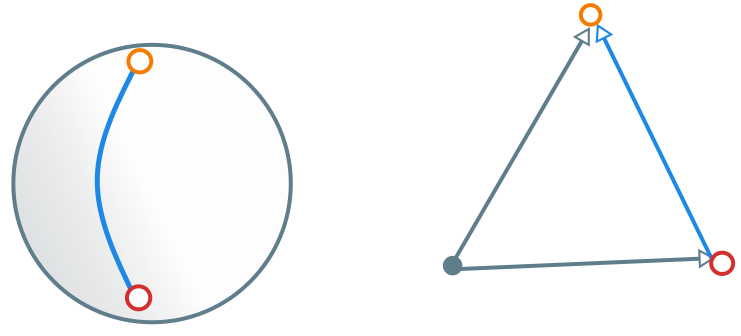
\includegraphics[width=\textwidth]{./sphere-shortest-path.png}
\caption{$(b - a)$ on a sphere versus the plane ($\R^2$). Red and
  orange are the words $b$, $a$. The path in blue for the sphere and the
  line in blue for the plane corresponds to the difference $(b - a)$. See
  how in the case of the plane, both the points as well as the difference can
  be represented by vectors. However, in the case of a sphere, this is
  not possible since there is no clean correspondence between a "path" and
  a point on the sphere.}
\end{figure}


\subsection{Generalizing \wtov: Distinction with differences}

Let us reformulate the fundamental operations performed with \wtov, in light
of our discussion above.

\begin{itemize}
\item Similarity: Given two words, find how similar they are in meaning. This is
     expressed as a dot product between the two vectors.
\item Analogy: Given two words, representing a sense of analogy \texttt{(king : man)},
      then a third word, representing the base of another analogous
      pair \texttt{(woman : ?)}, find the unknown word \texttt{?}
\end{itemize}


In our description of analogy, we deliberately describe the analogy operation
in two steps: first to provide an analogy \texttt{(king : man)}, and second
to provide the base of a new analogy \texttt{(woman : ? )}. As we shall see,
the mathematical generalization to Lie groups naturally contains this distinction;
Words such as \texttt{man, king, woman} become \emph{points} on the manifold,
while analogies such as \texttt{(king : man)} become \emph{paths} on the manifold.
This is not so strange, as this is exactly what happens in \wtov. We have
words such as \texttt{king, man, woman} which are vectors (elements of $\R^n$). 
On performing analogy \texttt{(a : b :: c : ?)}, we perform the vector
space operation $b - a + c$, which can be rearranged as $c + (b - a)$, which
is the base point $c$ to which we add the direction $(b - a)$.

% \begin{figure}
% 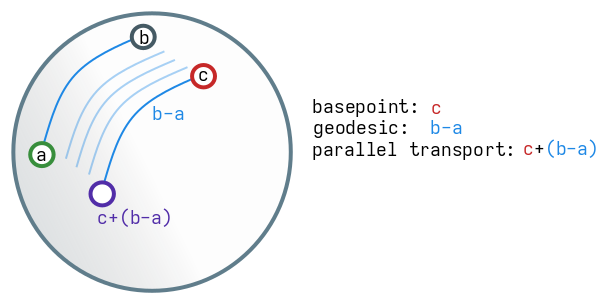
\includegraphics[width=0.8\textwidth]{./sphere-parallel-transport-geodesic.png}
% \caption{Computing analogy in curved spaces. Begin by choosing the analogous
% pair $(a : b)$. Compute the geodesic path between them, $(b - a)$. Transport
% the geodesic by using parallel transport to the basepoint $c$. This allows us
% to find the point $c +(b-a)$.}
% \end{figure}


\subsection{Lexical Semantics on a Symplectic Manifold}

\begin{figure}[H]
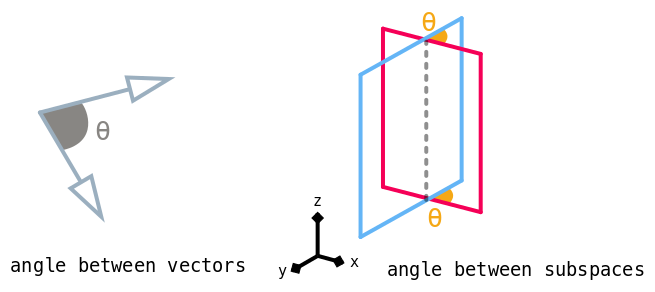
\includegraphics[width=\textwidth]{./symplectic.png}
\caption{Angle between subspaces. Here, we see that when we consider angle
 between words, it is only possible to consider a single sense direction. When
 we consider angles between subspaces, the subspace can capture multiple senses
 since it can extend into multiple directions.  The angle between the subspaces
 provides us our notion of similarity.}
\end{figure}

We first explain a modest generalisation of \wtov, the symplectic manifold,
after which we move on to the full generalisation. In the symplectic manifold,
we train pairs of vectors as our embedding representation, and use the
angle between their subspaces as the similarity measure.

\subsection{The Grassmanian: Generalizing \wtov to $n$-Dimensions}

The grassmanian Represents all $k$-dimensional subspaces of an $n$-dimensional
vector space. More importantly, the grassmanian is a \emph{lie group}; This means
that we can build analogues of the \wtov operations for the Grassmanian. Here,
we lay out a general theory of similarity and analogy, and use the theory to
develop our implementation of the Grassmanian.




\section{Training Mechanism}

\section{Results and Evaluation}

\section{Analysis}

\section{Contrastive Losses}

\subsection{The setting: Lie groups, Similarly, and Analogy}
A Lie group is a mathematical object that abstracts the ideas of "analogy"
and "similarity". These ideas are called as:
\begin{itemize}
\item \emph{Parallel transport}: given a base word and an analogy, find a word with the analogy we are interested in
\item \emph{Geodesic computation}: given two words, represent the analogy between the words.
\end{itemize}
% https://arxiv.org/abs/1902.09229
% http://svcl.ucsd.edu/publications/journal/2016/ggr/supplementary_material.pdf

\section{Related Work}

\section{Conclusion}

\chapter{Research direction II: Geometric algebras}


While not strictly in the realm of differential geometry, geometric algberas
are an interesting beast. Essentially, they answer the question:

\begin{quote}
    What if we could study vectors on equal footing with arbitrary subspaces?
\end{quote}

\section{Exterior Algebras}
We first define the \emph{exterior algebra of degree $2$} of a vector space $V$.
Intuitively, these represent \emph{oriented areas} of a space. Later,
we generalize these to volumes and hypervolumes.

Given a vector space $V$ of dimension $n$, we define a space $(\mathbf \Omega^2(V))$, called
as the exterior algebra of $V$ of degree 2. We can construct 
elements of $(\mathbf \Omega^2(V))$
by using an operator $(\wedge)$, defined by the following axioms:

\begin{align*}
    &\wedge: V \times V \rightarrow \mathbf \Omega^2(V) \\
    &\vec v \wedge \vec w  = -\vec w \wedge \vec v \qquad \text{(skew-symmetry)}\\
    &\forall \alpha, \beta, \gamma, \delta \in \R \quad \vec u, \vec v,\vec w, \vec x \in V, \\
    &\quad (\alpha \vec u + \beta \vec v) \wedge (\gamma \vec w + \delta \vec x) = 
        \alpha \gamma (\vec u \wedge \vec w) + 
        \alpha \delta (\vec u \wedge \vec x) + 
        \beta \gamma  (\vec v \wedge \vec w) +
         \beta \delta  (\vec v \wedge \vec x) \qquad \text{(bilinearity)}
\end{align*}

\section{Intuition of the definition of wedge products on $\R^2$}

From the above axioms, we can derive an intution for the wedge product in
$\mathbb R^2$. let us consider $\vec x, \vec y$ as unit basis vectors of $\R^2$.

We first show:
$[\vec x \wedge \vec x = - (\vec x \wedge \vec x) \implies 2 (\vec x \wedge \vec x = 0) \implies (\vec x \wedge \vec x = 0)]$.
Similarly, $(\vec y \wedge \vec y= 0)$. We also note that $\vec x \wedge \vec y = - \vec y \wedge \vec x$,
by using the skew-symmetry rule.


Now, we observe the value of $(v \wedge w)$ for a general $(v, w \in \R^2)$ and we
provide a geometric interpretation. We first write $\vec v, \vec w$ in terms
of the basis vectors $\vec x, \vec y$ as:
$(\vec v = \alpha \vec x + \beta \vec y), (\vec w = \gamma \vec x + \delta \vec y)$.
Next, we expand $(\vec v \wedge \vec w)$ as:

\begin{align*}
\vec v \wedge \vec w 
&= (\alpha \vec x + \beta \vec y) \wedge (\gamma \vec x + \delta \vec y) \\
&=       \alpha \gamma (\vec x \wedge \vec x) + 
        \alpha \delta (\vec x \wedge \vec y) + 
        \beta \gamma  (\vec y \wedge \vec x) + 
        \beta \delta  (\vec y \wedge \vec y)  \\
&= \alpha \gamma (0) + 
  \alpha \delta (\vec x \wedge \vec y)  +
  \beta \gamma (- \vec x \wedge \vec y) +
  \beta \delta (0) \\
&= (\alpha \delta - \beta \gamma)(\vec x \wedge \vec y)
\end{align*}

We know from 2D geometry that $(\alpha \delta - \beta \gamma)$ is the area
of the parallogram spanned by vectors $(\vec v, \vec w)$. Now, $\vec x \wedge \vec x = 0$
can be interpreted as "the parallelogram made up of two sides which are collinear has  0 area".
The fact $(\vec x \wedge \vec y = - \vec y \wedge \vec x)$ can be interpreted
as \emph{orientation}. We view $(\vec x \wedge \vec y)$ as an "anti-clockwise" 
orientation going from the positive $x$-axis (3 o clock) to the positive $y$-axis (12 o clock).
$(\vec y \wedge \vec x)$ is a clockwise orientation, going from the positive $y$-axis to
the positive $x$-axis.

\section{Generalizing exterior algebras to arbitrary dimensions}
Given a vector space $V$ of dimension $k$, we define the $k$-dimensional
exterior algebra space inductively as follows:

\begin{align*}
    &\Omega^k(n) \equiv \{ \vec x_1 \wedge \vec x_2 \wedge \dots \vec x_k \mid 
            \vec x_1, \vec x_2, \dots \vec x_k \in V \} \\
    & (\vec x_1 \wedge \dots \wedge x_k) = 
    sign(P)
    (\vec x_{P(1)} \wedge \vec x_{P(2)} \dots \wedge x_{P(k)})
    \qquad \text{(skew-symmetry)} \\
\end{align*}

where $(P: \{1, 2, \dots, k\} \rightarrow \{1, 2, \dots, k \})$ is a
permutation (bijection). $sign(P)$ is $+1$ if the permutation is an
even permutation (contains an even number of swaps), and $-1$ if it
is an odd permutation (contains an odd number of swaps) 

\begin{align*}
    &(\vec x_1 \wedge \dots (\alpha \vec y_1 + \beta \vec y_2) \wedge \vec x_k) = \\
    &\qquad \alpha (\vec x_1 \wedge \dots \wedge \vec y_1 \wedge \dots \wedge \vec x_k) +
    \beta (\vec x_1 \wedge \dots \wedge  \vec y_2 \wedge \dots \wedge \vec x_k)
    \qquad \text{(multi-linearity)}
\end{align*}

Note that this clearly extends the situation as described in $2D$ to $nD$.


\section{Geometric algebra}
\newcommand{\G}{\mathbb{G}}

The geometric algebra of a vector space $V$ over the reals $\R$ of dimension $n$
is called as $\G(V)$. $\G(V)$ contains
all \emph{formal linear combinations} of elements from
$\left( \R, V, \Omega^2(V), \Omega^3(V), \dots \Omega^n(V) \right)$.
For example, if we consider the space $\G(\R^2)$, an element of this space 
is  $(2 -3 \vec x + 4 \vec y + 5 \vec x \wedge \vec y)$. 

This is a unique space, because it allows us to combine objects such as 
scalars, vectors, areas, volumes, etc. This is the power that we shall exploit
to model a wide variety of situations.

In general, if the vector space $V$ is of dimension $n$, then the geometric
algebra $\G(V)$ will have dimension $2^n$, since it will contain as a basis
all possible collections of subspaces.


\section{The philosophy of geometric algebra}
In general, within vector spaces, vectors are privileged. Subspaces on the
other hand are defined with equations: for example, in $3D$, the subspace
spanned by the $\vec x, \vec y$ axes would be
$span(\vec x, \vec y) =
\{ \lambda_x \vec x  + \lambda_y \vec y \mid \lambda_x, \lambda_y \in \R \}$
This is a \emph{set of vectors}, and not an \emph{element of the vector space}.

In a geometric algebra, we would represent the subspace (roughly) as $(\vec x \wedge \vec y)$.
This allows us to treat vectors, scalar, volumes, and hypervolumes on
equal footing, and develop a theory that includes all of these objects.

It also provides a \emph{geometric product}, that allows us to easily relate
the regular \emph{inner product} to the \emph{exterior product}, thereby
creating a unifying theory of vectors and all differential forms.

\subsection{The geometric product}

We first define the geometric product for vectors:
\begin{align*}
    ab \equiv (a \cdot b) + (a \wedge b)
\end{align*}


\subsection{Construction: A non-commutative, bilinear structure for geometric algebra}

We define a non-commutative, bilinear structure
$\left(\braket{\cdot}{\cdot}: \G(V) \times \G(V) \rightarrow \R\right)$. We
define the effect on the basis elements, and then extend it to the
full space. Let the basis of $V$ be $\{ b_1, b_2, \dots, b_k \}$.


\begin{align*}
\braket{b_{i_1} \wedge b_{i_2} \wedge \dots \wedge b_{i_n}}{c_{j_1} \wedge c_{j_2} \wedge \dots \wedge c_{j_m}}
\equiv
\begin{cases}
1 & span(b_{i_1}, b_{i_2}, \dots, b_{i_n}) \subseteq span(c_{j_1}, c_{j_2}, \dots, c_{j_m}) \\
0 & \text{otherwise}
\end{cases}
\end{align*}

Then we extend this multi-linearly to the full space, since we have defined its
action on the basis.

\begin{example}
\begin{align*}
&\braket{2 + 3\vec x + 4 \vec x \wedge \vec y}{4\vec y} \\
&= \braket{2}{4\vec y} +
 \braket{3\vec x}{4\vec y} +
 \braket{4 \vec x \wedge \vec y}{2 \vec x \wedge \vec y} \\
&= (2 \cdot 4)\braket{1}{\vec y} + 
   (3 \cdot 4) \braket{\vec x}{\vec y} + 
   (4 \cdot 4) \braket{\vec x \wedge \vec y}{\vec y} \\
&= 8 (1) + 12 (0) + 16 (0) = 8
\end{align*}
\end{example}
Note that $(\braket{\vec x}{\vec y} = 0)$, since the space spanned by $\vec x$
is not contained in the space spanned by $\vec y$. Similarly, 
$(\braket{\vec x \wedge \vec y}{\vec y} = 0)$, since the subspace spanned by
$(\vec x, \vec y)$ is strictly bigger than the subspace spanned by $(\vec y)$.


This dot product structure captures the asymmetric notion of "containment":
$\braket{b}{c} \neq 0$ iff the span of $b$ is contained in the span of $c$.
This allows us to model situations where we wish to have a notion of containment
\emph{across subspaces} of a given space.

%--------------------------------------------------------
%%% Optional appendix
%\appendix
%\chapter{}
%\label{}

%--------------------------------------------------------
% Recommended 'Related Publication'
\chapter*{Related Publications}
\label{ch:relatedPubs}
\input{relatedPapers.tex}

%--------------------------------------------------------

\bibliographystyle{latex8}
%\bibliography{References,Introduction/References} % To include one or more reference.bib files
\bibliography{sampleBib} 

\end{document}
